\section{BIOS}
\label{sec:bios}
This section was written by Vincent Lee, Ian Juch, and Albert Magyar.

\subsection{Background}
For the first checkpoint we have provided you a BIOS written in C that your processor is
instantiated with. BIOS stands for Basic Input/Output System and forms the bare bones of the
CPU system on initial boot up. The primary function of the BIOS is to locate, and initialize the
system and peripheral devices essential to the PC operation such as memories, hard drives, and
the CPU cores.

Once these systems are online, the BIOS locates a boot loader that initializes the operating
system loading process and passes control to it. For our project, we do not have to worry about
loading the BIOS since the FPGA eliminates that problem for us. Furthermore, we will not deal
too much with boot loaders, peripheral initialization, and device drivers as that is beyond the
scope of this class. The BIOS for our project will simply allow you to get a taste of how the
software and hardware layers come together.

The reason why we instantiate the memory with the BIOS is to avoid the problem of
bootstrapping the memory which is required on most computer systems today. Throughout the
next few checkpoints we will be adding new memory mapped hardware that our BIOS will
interface with. This document is intended to explain the BIOS for checkpoint 1 and how it
interfaces with the hardware. In addition, this document will provide you pointers if you wish to
modify the BIOS at any point in the project.

\subsection{Loading the BIOS}
For the first checkpoint, the BIOS is loaded into the Instruction memory when you first build it.
As shown in the Checkpoint 1 specification, this is made possible by instantiating your
instruction memory to the BIOS file by building the block RAM with the \verb|bios151v3.hex| file. If you
want to instantiate a modified BIOS you will have to change this .hex file in your block RAM
directory and rebuild your design and the memory.

To do this, simply cd to the \verb|software/bios151v3| directory and make the .hex file by running
“make”. This should generate the .hex file using the compiler tailored to our ISA. The
block RAM will be instantiated with the contents of the .hex file.
When you get your design to synthesize and program the board, open up screen using the
same command from Lab 5:

\verb|screen $SERIALTTY 115200|

or

\verb|screen /dev/ttyUSB0 115200|

Once you are in \verb|screen|, if you CPU design is working correctly you should be able to hit Enter
and a carrot prompt \verb|'>'| will show up on the screen. If this doesn’t work, try hitting the reset
button on the FPGA. If you can’t get the BIOS
carrot to come up, then your design is not working and you will have to fix it.

\subsection{Loading Your Own Programs}
The BIOS that we provide you is written so that you can actually load your own programs for
testing purposes and benchmarking. Once you instantiate your BIOS block RAM with the
\verb|bios151v3.hex| file and synthesize your design, you can transfer your own program files over the
serial line.

To load you own programs into the memory, you need to first have the .hex file for the program
compiled. You can do this by copying the software directory of one of our C programs folders in
/software directory and editing the files. You can write your own MIPS program by writing
test code to the .s file or write your own c code by modifying the .c file.
Once you have the .hex file for your program, impact your board with your design and run:

\verb|hex_to_serial <file name> <target address>|

The \verb|<file name>| field corresponds to the .hex file that you are to uploading to the instruction
memory. The \verb|<target address>| field corresponds to the location in memory you want to write
your program to.

Once you have uploaded the file, you can fire up screen and run the command:

\verb|jal <target hex address>|

Where the \verb|<target hex address>| is where you stored the location of the hex file over
serial. Note that our design does not implement memory protection so try to avoid storing your
program over your BIOS memory. Also note that the instruction memory size for the first
checkpoint is limited in address size so large programs may fail to load.
The jal command will change the PC to where your program is stored in the instruction
memory.

\subsection{The BIOS Program}
The BIOS itself is a fairly simple program and composes of a glorified infinite loop that waits for
user input. If you open the \verb|bios151v3.c| file, you will see that the main method composes of a
large for loop that prints a prompt and gets user input by calling the \verb|read_token| method.
If at any time your program execution or BIOS hangs or behaves unexpected, you can hit the
reset button on your board to reset the program execution to the main method.
The \verb|read_token| method continuously polls the UART for user input from the keyboard until it
sees the character specified by ds. In the case of the BIOS, the termination character
\verb|read_token| is called with is the 0xd character which corresponds to Enter.
The \verb|read_token| method will then return the values that it received from the user.

\begin{figure}[H]
  \centering
  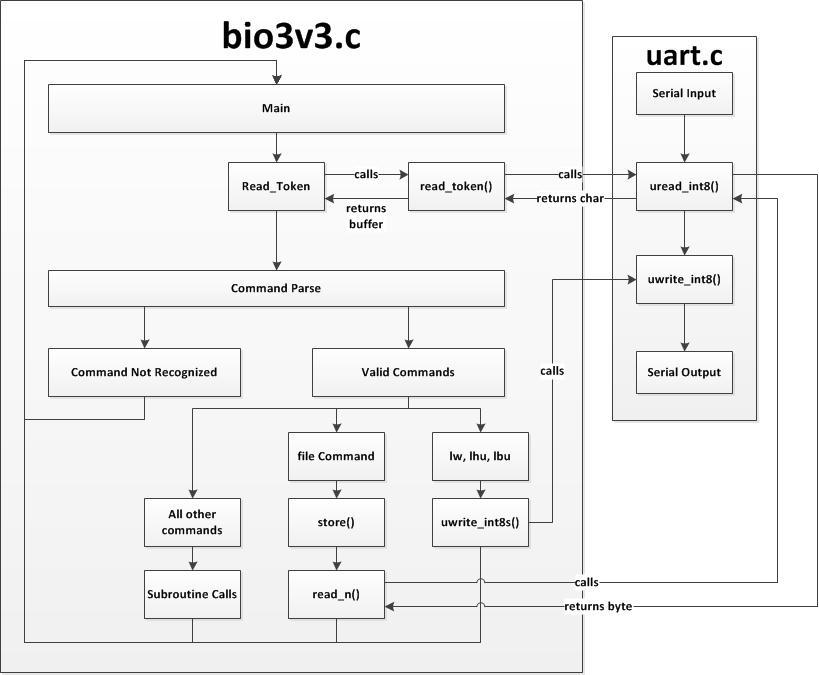
\includegraphics[width=0.7\textwidth]{figs/bios_flow.png}
  \caption{BIOS Execution Flow}
\end{figure}

The buffer returned from the \verb|read_token| method with the user input is then parsed by
comparing the returned buffer against commands that the BIOS recognizes. If the BIOS parses a
command successfully it will execute the appropriate subroutine or commands. Otherwise it
will tell you that the command you input is not recognized.
If you want to add commands to the BIOS at any time in the project, you will have to add to the
comparisons that follow after the \verb|read_token| subroutine in the BIOS.

\subsection{The UART}
You will notice that some of the BIOS execution calls will call subroutines in the uart.c file
which takes care of the transmission and reception of byte over the serial line.
The uart.c file contains three subroutines. The first subroutine, \verb|uwrite_int8| executes a
UART transmission for a single byte by writing to the output data register. The second
subroutine \verb|uwrite_int8s| allows you to process an array of type \verb|int8_t| or chars and send
them over the serial line. The third routine \verb|uread_int8| polls the UART for valid data and
reads a byte from the serial line.

In essence, these three routines are operating the UART on your design from a software view
using the memory mapped I/O. Therefore, in order for the software to operate the memory
map correctly, the \verb|uart.c| module must store and load from the correct addresses as defined
by out memory map. You will find the necessary memory map addresses in the uart.h file that
conforms to the design specification.

\subsection{Command List}
The following commands are built into the BIOS that we provide for you. All values are
interpreted in hexadecimal and do not require any radix prefix (ex. ``0x''). Note that there is not
backspace command.

\verb|jal <hexadecimal address>| - Moves program execution to the specified address

\verb|lw <hexadecimal address>| - Displays word at specified address to screen

\verb|lhu <hexadecimal address>| - Displays half at specified address to screen

\verb|lbu <hexadecimal address>| - Displays byte at specified address to screen

\verb|sw <value> <hexadecimal address>| - Stores specified word to address in memory

\verb|sh <value> <hexadecimal address>| - Stores specified half to address in memory

\verb|sb <value> <hexadecimal address>| - Stores specified byte to address in memory

There is another command file in the main() method that is used only when you execute
\verb|hex_to_serial|. When you execute \verb|hex_to_serial|, your workstation will initiate a byte
transfer by calling this command in the BIOS. Therefore, don’t mess with this command too
much as it is one of the more critical components of your BIOS.

\subsection{Adding Your Own Features}
Feel free to modify the BIOS code if you want to add your own features during the project for
fun or to make your life easier. If you do choose to modify the BIOS, make sure to preserve
essential functionality such as the I/O and the ability to store programs. In order to add
features, you can either add to the code in the \verb|bios151v3.c| file or create your own c source and
header files. Note that you do not have access to standard c libraries so you will have to add
them yourself if you need additional library functionality.

\newpage
